\part{Capitulo 5}

\section{Precipitación}

Las Precipitación son las aguas meteoricas que provienen de la humedad atmosférica y que caen a la superficie terrestre.\\
Incluye: 
\begin{itemize}
    \item Lluvia
    \item Nieve
    \item Granizo
    \item Rocío
\end{itemize}

Esta se considera como la \textcolor{blue}{lamina de agua} que se acumula sobre una superficie dada en un tiempo determinado y si toda la precipitacion permaneciera en el mismo lugar.\\
Esta se mide en mm (SI) y en pulgadas (USA).\\

\begin{description}
    \item[Antes de caer al suelo:] \textbf{METEOROLOGÍA}
    \item[Después de caer al suelo:] \textbf{HIDROLOGÍA}
\end{description}

\section{Mecanismos de formacion de la precipitación}

Para esto se necesita que una masa de agua en la atmosfera ascienda, se enfrie y se condense.\\
Los tres mecanismos son:
\begin{itemize}
    \item \textbf{Mecanismo frontal} : Aire caliente es elevado sobre una masa fria luego de formarse un frente.
    \item \textbf{Mecanismo orografico} : El aire es elevado por accidentes geograficos (ej. cordones montañosos).
    \item \textbf{Mecanismo convectivo} : Masas de aire arrastradas hacia arriba por accion convectiva luego de calentamineto superficial.
\end{itemize}

\subsection{Mecanismo frontal}

Este fenómeno puede ocurrir por dos tipos de frentes: 
\begin{itemize}
    \item \textbf{Frente frío}: Aire frío irrumpe sobre aire caliente, lo que provoca un ascenso de aire caliente. (cubre menor área, 60 a 80 km)
    \item \textbf{Frente caliente}: Aire caliente avanza sobre aire frío, lo que provoca que el aire caliente ascienda. (cubre una mayor área, 100 a 300 km)
\end{itemize}

\begin{figure}[!htbp]
    \centering
    \begin{minipage}{0.35\textwidth} % Aumenta un poco el ancho si es necesario
        \centering
        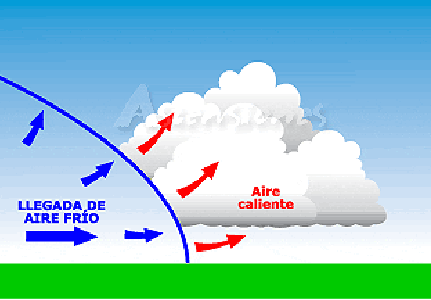
\includegraphics[width=\textwidth]{imagenes/frente_frio.png}
        \label{fig:frente_frio}
    \end{minipage}
    \hspace{0.05\textwidth} % Controla el espacio entre las dos imágenes
    \begin{minipage}{0.35\textwidth}
        \centering
        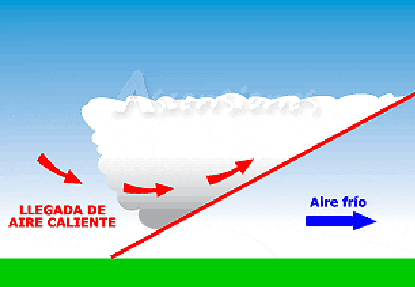
\includegraphics[width=\textwidth]{imagenes/frente_caliente.png}
        \label{fig:frente_caliente}
    \end{minipage}
\end{figure}

\newpage
\subsection{Mecanismo orografico}

Este fenómeno se produce cuando una masa de aire húmeda y caliente es forzada a ascender por una barrera geografica.\\
Suele ser de baja intensidad, pero importnate cantidad.\\

\begin{figure}[h]
    \centering
    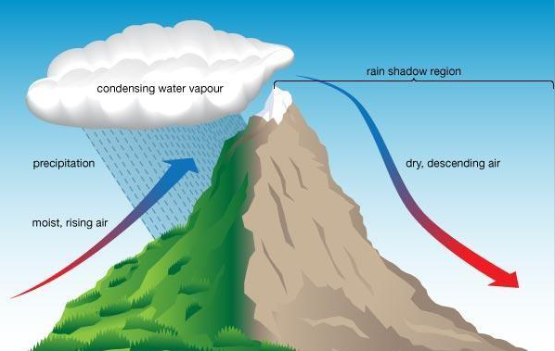
\includegraphics[width=0.4\textwidth]{imagenes/pp_orografica.png}
    \label{pp_orografica}
\end{figure}

\subsection{Mecanismo convectivo}   

En este fenómeno, el aire caliente y húmedo asciende por convección, lo que provocaque la atmosfera se vuelva inestable. Esto lleva a que el ascenso casi vertical del aire se expanda y se enfri por e cambio de presion. Esto lleva a que el aire alcance la temperatura de rocío y se condense.\\
En este caso se crean nubes extensas con precipitaciones intensas y de corta duración.\\

\begin{figure}[h]
    \centering
    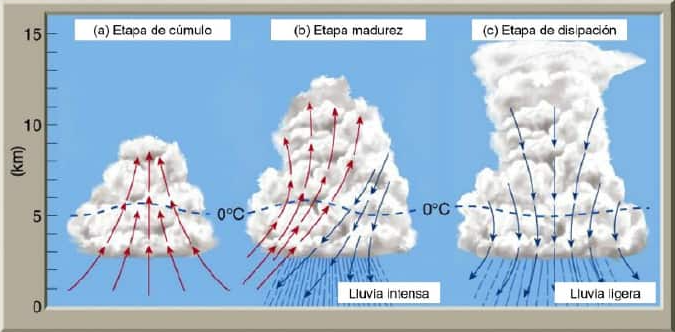
\includegraphics[width=0.4\textwidth]{imagenes/pp_convectiva.png}
    \label{pp_convectiva}
\end{figure}

\section{Medición de la precipitación}

El instrumento basico que se utiliza es el \textbf{pluviometro}, que es un recipiente cilindrico con una escala graduada en su interior, este se suele medir en mm de altura de agua.\\

\begin{figure}[h]
    \centering
    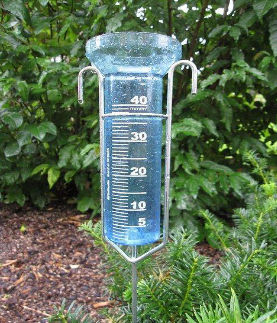
\includegraphics[width=0.2\textwidth]{imagenes/pluviometro.png}
    \label{pluviometro}
\end{figure}

Aunque si se busca una informacion continua y mas detallada se utilizan los \textbf{pluviografos}, que son pluviometros con un mecanismo de registro automatico, que se vacian para seguir midiendo en un periodo de tiempo.\\

\begin{figure}[!htbp]
    \centering
    \begin{minipage}{0.15\textwidth} 
        \centering
        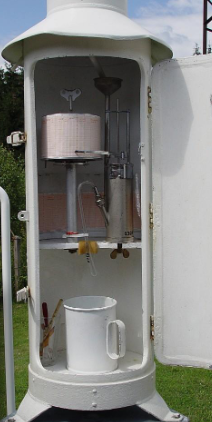
\includegraphics[width=\textwidth]{imagenes/pluviografo.png}
        \label{pluviografo}
    \end{minipage}
    \hspace{0.05\textwidth} % Controla el espacio entre las dos imágenes
    \begin{minipage}{0.2\textwidth}
        \centering
        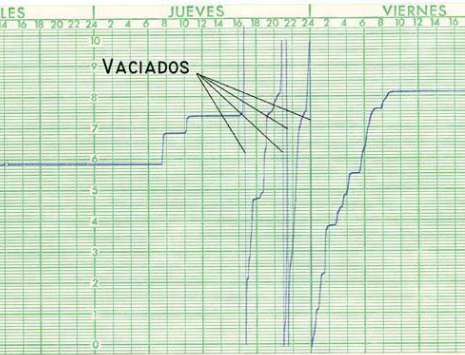
\includegraphics[width=\textwidth]{imagenes/grafico_pluviografo.png}
        \label{grafico_pluviografo}
    \end{minipage}
\end{figure}

\subsection{Errores en la medición}

\begin{itemize}
    \item \textbf{Errores de lectura}: como la lectura de la reglilla o lectura de graficos.
    \item \textbf{Errores instrumentales}: como la evaporación del agua, el viento, la obstrucción del embudo, etc.
    \item \textbf{Errores provenientes de la exposicion e instalacion}: Como el efecto del viento, la altura de la instalacion, la obstruccion de la lluvia, etc.
\end{itemize}

\section{Procesamiento de datos de pluviometricos}

Esto busca generar estadisticas de la precipitacion para caracterizar el regimen de precipitaciones a escala diaria, mensual, anual, segun sea necesario.\\
Previo al uso de los datos de debe someter a un ajuste para: 

\begin{itemize}
    \item \textbf{Rellenar y/o completar datos faltantes}: para esto se utiliza el metodo del modelo pluviometrico o correlaciones y/o regresiones.
    \item \textbf{Establecer su calidad y consistencia}: para esto se utilizan el metodo de la curva doble acumulada (CDA).
\end{itemize}

\subsection{Estimacion de datos faltantes}

Es frecuente que falten algunos datos para ciertos dias, meses o años, por lo que para el relleno de valores aislados se recomienda el uso de l menos tres estaciones de las estaciones mas cercanas.

\subsubsection{Modelo pluviometrico (M)}

Es el promedio aritmetico durante un cierto periodo de tiempo (normalmente 30 años) de las precipitaciones anuales registradas en una region.\\

\begin{equation}
    M = \frac{1}{N} \sum_{i=1}^{N} P_{anuales}
\end{equation}

\subsubsection{Metodo del modulo pluviometrico}

\begin{itemize}
    \item Si el modulo pluviometrico de la estacion difiere en menos de un 10 \% de las estaciones vecinas: \\
    \begin{equation}
        P_X = \frac{1}{3}(P_A + P_B + P_C)
    \end{equation}
    \item Si el modulo pluviometrico de la estacion difiere en mas de un 10 \% de las estaciones vecinas: \\
    \begin{equation}
        \frac{P_X}{M_X} = \frac{1}{3}(\frac{P_A}{M_A} + \frac{P_B}{M_B} + \frac{P_C}{M_C})
    \end{equation}
\end{itemize}

\subsubsection{Correlaciones o regresiones lineales}

Sirve para correlacionar la informacion pluviometrica con la registrada en estaciones vecinas para un mismo año, mes o dia.\\

\begin{figure}[H]
    \centering
    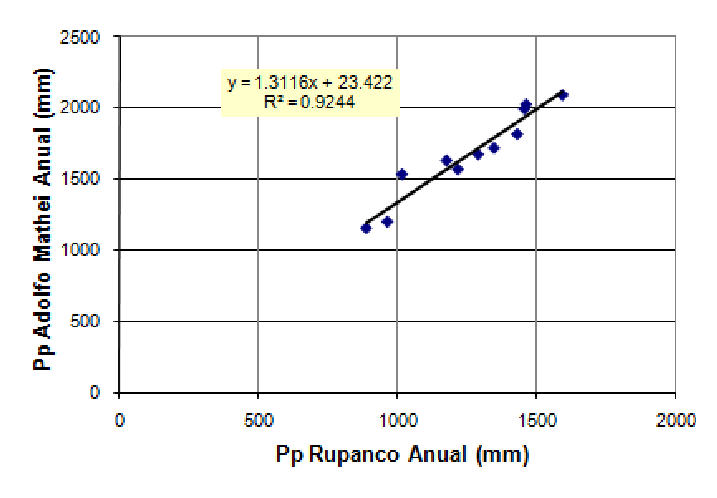
\includegraphics[width=0.28\textwidth]{imagenes/correlacion_anual.png}
    \label{correlacion}
\end{figure}

\subsubsection{Consistencia de las estadisticas pluviometricas \\ Curva doble acumulada (CDA)}

Este metodo se utiliza para verificar la consistencia de los datos pluviometricos, para esto se grafican las precipitaciones acumuladas en un periodo de tiempo y se comparan con las precipitaciones acumuladas de varias estaciones cercanas.\\

La estacion patron, en los posible, debe calcularse como el promedio de 10 estaciones cercanas con estadisticas completas (o las maximas posibles).\\

Para esto se grafica la precipitacion anual acumulada de la estacion de analisis versus el valor acumulado de una estacion patron.\\

Este proceso es iterativo, partiendo con un patron que contenga todas las estaciones posibles y eliminado las que no cumplan con la consistencia.\\

Lo que deriba en que se la zona es pluviometricamente homogenea, el grafico llegara a una unica tendecia.\\

Si la zona es \textbf{homogenea}, el grafico sera una recta de pendiente $\alpha$ que pasa por el origen: \\
\begin{figure}[H]
    \centering
    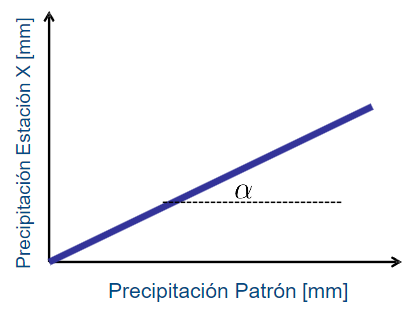
\includegraphics[width=0.3\textwidth]{imagenes/cda_homo.png}
    \label{cda_homo}
\end{figure}

Si la zona es \textbf{no homogenea}, el grafico tendra cambios de pendiente, por lo que se debe homogeneizar mediante la conveccion respecto al periodo mas reciente:

\begin{equation}
    P_{\text{ajustada}} = P_{\text{observada}} \cdot \frac{M_{\text{aj}} \, (\text{Periodo reciente})}{M_{\text{obs}} \, (\text{periodo a corregir})}
\end{equation}

\begin{figure}[H]
    \centering
    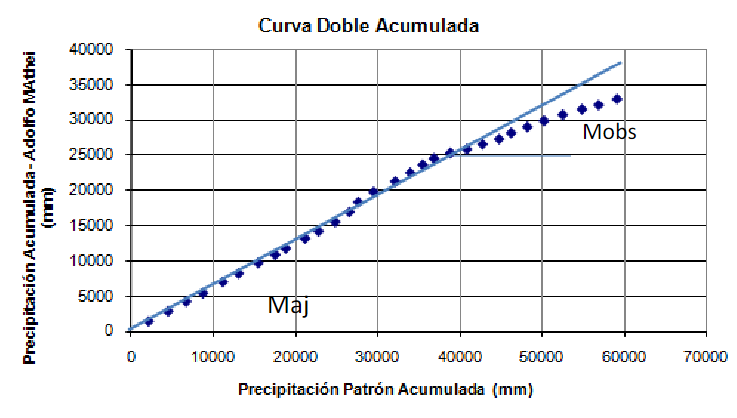
\includegraphics[width=0.3\textwidth]{imagenes/cda_no_homo.png}
    \label{cda_no_homo}
\end{figure}

\subsubsection{Relleno de datos usando curva CDA}

Este metodo se puede utilizar para completar datos no observados. \\

\begin{equation}
    P_X = P_a \frac{M_x}{M_a}
\end{equation}

donde: 
\begin{itemize}
    \item $P_x$ = precipitación no medida en estación X durante año n.
    \item $M_x$ = pendiente de la recta masica para estacion X.
    \item $P_a$ = precipitacion medida en estacion A vecina durante año n.
    \item $M_a$ = pendiente de la recta masica para estacion A.
\end{itemize}

\subsection{Precipitación media}

Normalmente es necesario establecer una magnitud de la precipitacion media de cierta region. Para esto existen 3 modos alternativos: \\

\begin{itemize}
    \item Media aritmetica
    \item Metodo de los poligonos de Thiessen
    \item Metodo de las Isoyetas
    \item Uso de productos grillados
\end{itemize}

\subsubsection{Media aritmetica}

Corresponde al promedio de todas las estaciones del area de estudio. Este metodo es el mas simple, pero el menos preciso.\\

\begin{equation}
    \overline{P} = \frac{1}{N} \sum_{i=1}^{N} P_i
\end{equation}

\begin{figure}[H]
    \centering
    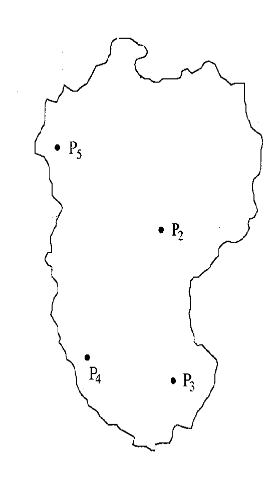
\includegraphics[width=0.15\textwidth]{imagenes/media_aritmetica.png}
    \label{media_aritmetica}
\end{figure}

\subsubsection{Metodo de los poligonos de Thiessen}

Corresponde a un promedio ponderado de las precipitaciones de las distintas estaciones de la region. El factor de ponderacion corresponde a la magnitud relativa de la area de influencia de cada estacion y el area total.\\

\begin{equation}
    \overline{P} = \sum_{i=1}^{N} P_i \cdot \frac{A_i}{A_T}
\end{equation}

\begin{figure}[H]
    \centering
    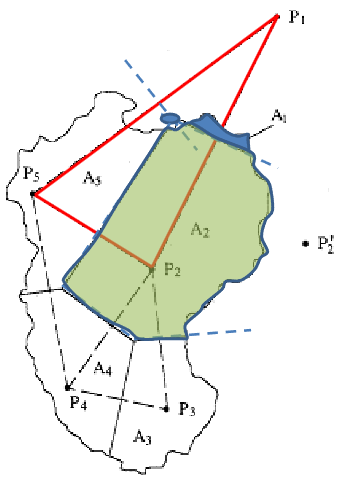
\includegraphics[width=0.15\textwidth]{imagenes/poligonos_thiessen.png}
    \label{thiessen}
\end{figure}

Las áreas de influencia se obtienen al determinar los polígonos que resultan de la intercepción de las simetrales en una red de triángulos que unen las estaciones.

\subsubsection{Metodo de las Isoyetas}

Este metodo consiste en trazar lineas que unen puntos de igual precipitacion.\\
Estas se trazan mediante la interpolacion y permite incluir estaciones fuera de la region pero cercanas.\\

\begin{equation}
    \overline{P} = \sum_{i=1}^{N_{bandas}} P_i \cdot (\frac{A_i}{A_T})
\end{equation}

Donde:
\begin{itemize}
    \item $P_i$ = precipitacion media de la banda i.
    \item $A_i$ = area de la banda i.
    \item $A_T$ = area total de la region.
\end{itemize}

\begin{figure}[H]
    \centering
    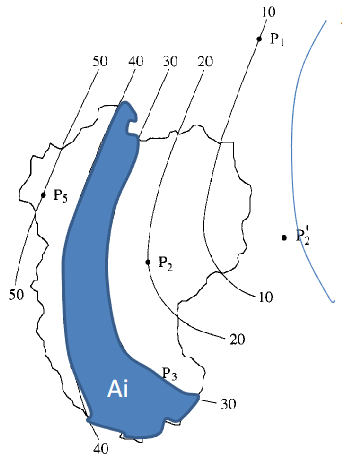
\includegraphics[width=0.15\textwidth]{imagenes/isoyetas.png}
    \label{isoyetas}
\end{figure}

\subsubsection{Uso de productos grillados}

Este metodo consiste en el uso de productos de precipitacion que se obtienen mediante el uso de satelites, radares, etc.\\

\begin{figure}[H]
    \centering
    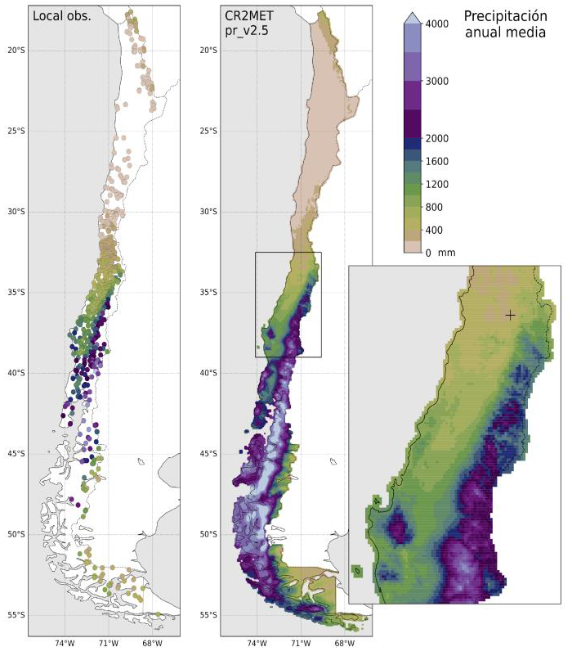
\includegraphics[width=0.15\textwidth]{imagenes/productos_grillados.png}
    \label{productos_grillados}
\end{figure}

\section{Presentación de datos de una estacion}

Para presentar los datos de una estacion se deben calcular las precipitaciones medias mensuales y anuales, ademas de incluir los siguientes parametros:\\

\begin{itemize}
    \item Valores minimos y maximos de precipitacion mensual.
    \item Desviacion estandar de la precipitacion mensual.\\
    \begin{equation}
        \sigma = (\frac{\sum_{}^{} (X_i - X_{med})^2}{N-1})^{(1/2)}
    \end{equation}
    \item Coeficiente de variacion de la precipitacion mensual.\\
    \begin{equation}
        CV = \frac{\sigma}{X_{med}}
    \end{equation}
\end{itemize} 

\section{Precipitación maxima}

Desde el punto de vista ingeneril nos interesa:

\begin{equation}
    i = \frac{dP}{dt}
\end{equation}

Que es la intensida de la precipitacion, que en SI es en mm/hora.\\

\begin{figure}[H]
    \centering
    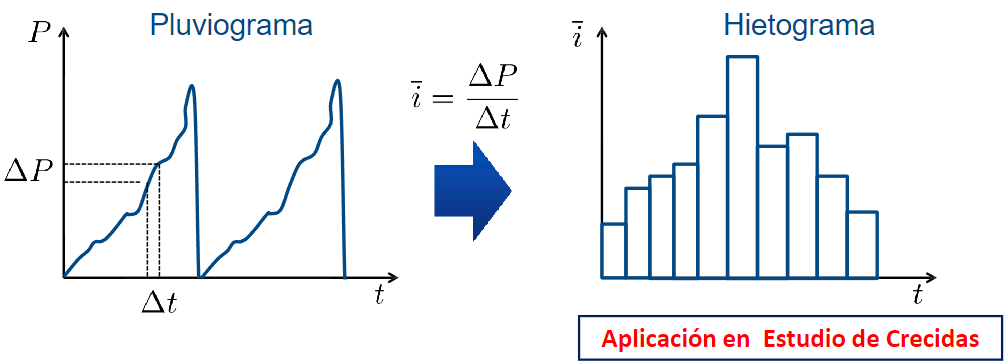
\includegraphics[width=0.7\textwidth]{imagenes/hietograma.png}
    \label{hietograma}
\end{figure}

Un hietograma es una curva representativa de la variacion de la intensidad de precipitacion en el tiempo.

\newpage
\subsection{Curva de intensidad-duracion}

Cada tormenta presenta su propia curva I-D.\\
Esta curva representa la intensidad de la precipitacion en funcion de la duracion de la misma.\\

\begin{figure}[!htbp]
    \centering
    \begin{minipage}{0.15\textwidth} 
        \centering
        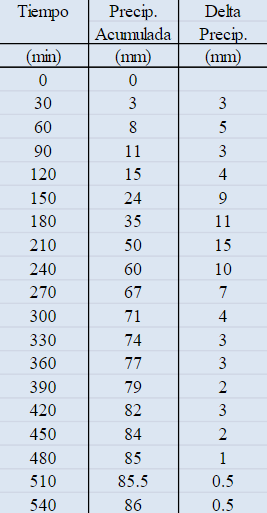
\includegraphics[width=\textwidth]{imagenes/datos_i_d.png}
        \label{datos_i_d}
    \end{minipage}
    \hspace{0.05\textwidth} % Controla el espacio entre las dos imágenes
    \begin{minipage}{0.3\textwidth}
        \centering
        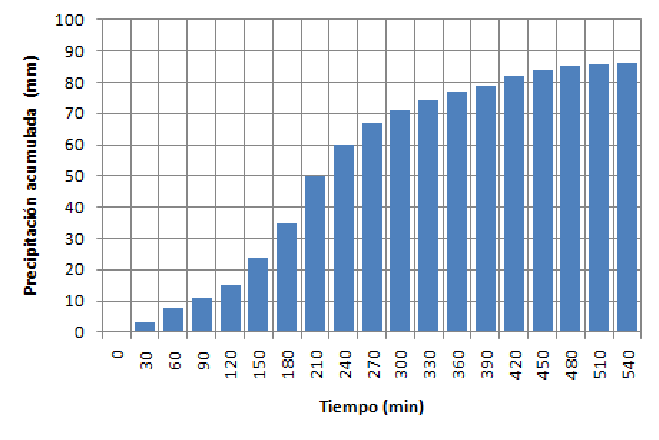
\includegraphics[width=\textwidth]{imagenes/histograma_i_d.png}
        \label{histograma_i_d}
    \end{minipage}
\end{figure}

Para el calculo de la curva intesidad-duracion:

\begin{figure}[H]
    \centering
    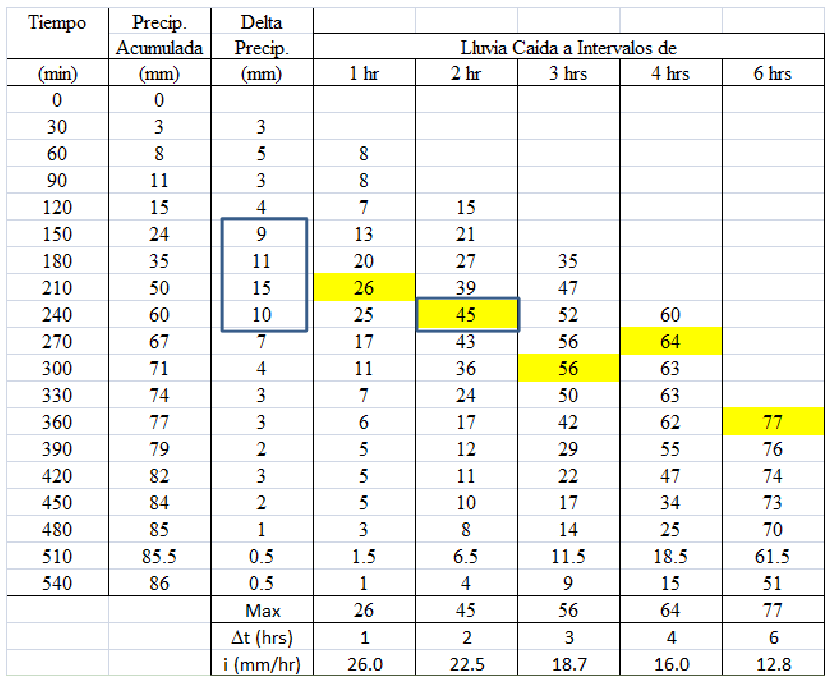
\includegraphics[width=0.5\textwidth]{imagenes/calculo_i_d.png}
    \label{calculo_i_d}
\end{figure}

Luego la curva intensidad-duracion se obtiene mediante la interpolacion de los puntos obtenidos.\\

\begin{figure}[H]
    \centering
    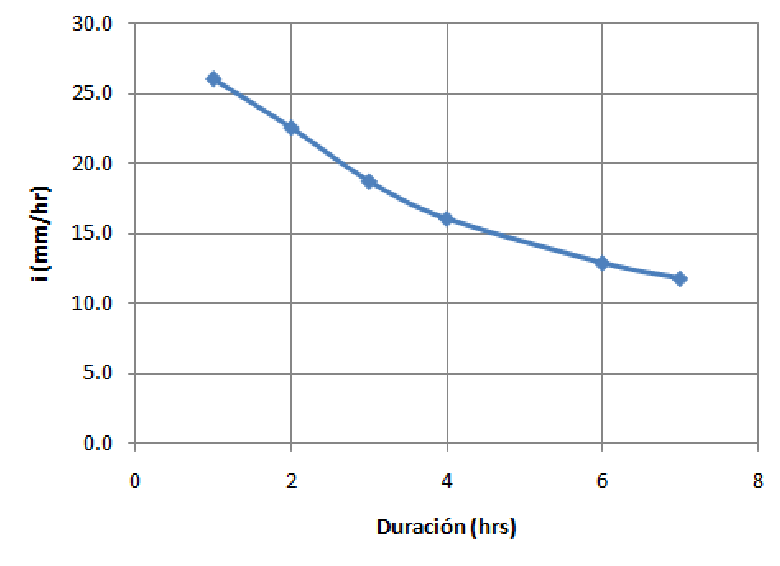
\includegraphics[width=0.4\textwidth]{imagenes/curva_i_d.png}
    \label{curva_i_d}
\end{figure}

\subsubsection{Curva de intensidad-duracion (forma simplificada)}

Para el calculo de la curva de intensidad-duracion de forma simplificada se utiliza la formula de Grunsky:

\begin{equation}
    i_t = i_{24} \sqrt{\frac{t}{24}} [mm/h]
\end{equation}

\subsection{Curva de intensidad-duracion-frecuencia (IDF)}

Esta curva representa la intensidad de la precipitacion en funcion de la duracion de la misma y la frecuencia de ocurrencia.\\

\begin{figure}[H]
    \centering
    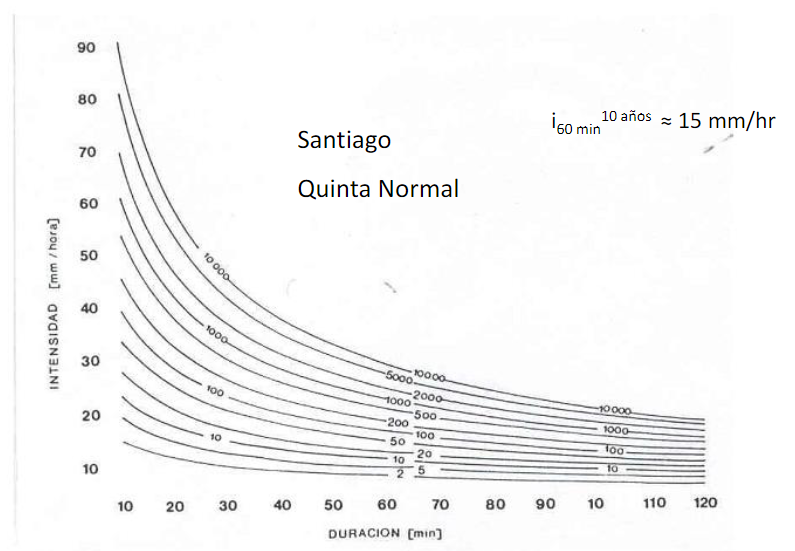
\includegraphics[width=0.4\textwidth]{imagenes/curva_idf.png}
    \label{curva_idf}
\end{figure}

Para una estimacion a partir de datos de lluvia diarios se utiliza la siguiente formula:

\begin{equation}
    P_t^T = K \cdot CD_t \cdot CF^T \cdot P_{maxd}^T
\end{equation}

Donde:
\begin{itemize}
    \item $P_t^T$ = precipitacion maxima de duracion t y periodo de retorno T [mm].
    \item $K$ = factor de correccion ($P_{\text{p maxd}}$ a $P_{\text{p max}}$ en 24 horas).\\ Usualmente K = 1,10
    \item $CD_t$ = coeficiente de duracion para duracion t.
    \item $CF^T$ = coeficiente de frecuencia asociado al periodo de retorno T.
    \item $P_{maxd}^T$ = precipitacion maxima diaria en t años [mm].
\end{itemize}

En caso de que t sea menor que 1 hora se utiliza la formula de Bell:

\begin{equation}
    P_t^T = (0.21 \cdot ln(T) + 0.52)(0.54 \cdot t^{0.25} - 0.5)P_{60}^t
\end{equation}

Donde:
\begin{itemize}
    \item $P_{t}^T$ = precipitacion de duracion t (minutos) y periodo de retorno T (años).
\end{itemize}